\documentclass{article}
\usepackage{fancyhdr}
\usepackage{lipsum}  
\usepackage{listings} 
\usepackage{xcolor}   
\usepackage{amsmath}
\usepackage{enumitem}
\usepackage{graphicx}
\usepackage{caption}
\usepackage{verbatim}

% Define macros for title and author
\newcommand{\thetitle}{STAT 641 \\ Homework 7}
\newcommand{\theauthor}{Keegan Smith}

\title{\thetitle}
\author{\theauthor}

\pagestyle{fancy}
\fancyhf{}  % Clear all header and footer fields
\fancyhead[L]{\nouppercase{\rightmark}}
\fancyhead[C]{\thetitle}  % Title in the center
\fancyhead[R]{\theauthor}  % Your name on the right

\lstset{ %
  backgroundcolor=\color{lightgray},   % choose the background color
  basicstyle=\ttfamily\small,          % size of fonts used for the code
  keywordstyle=\color{blue},           % color for keywords
  commentstyle=\color{green},          % color for comments
  stringstyle=\color{red},             % color for strings
  numbers=left,                        % where to put the line-numbers
  numberstyle=\tiny\color{gray},       % style for line-numbers
  stepnumber=1,                        % the step between two line-numbers
  numbersep=5pt,                       % how far the line-numbers are from the code
  frame=single,                        % adds a frame around the code
  rulecolor=\color{black},             % frame color
  breaklines=true,                     % automatic line breaking
  breakatwhitespace=false,             % automatic breaks should only happen at whitespace
  showspaces=false,                    % don't show spaces in the code
  showstringspaces=false,              % don't show spaces in strings
  showtabs=false,                      % don't show tabs in the code
}

\begin{document}

\maketitle
\section*{Problem 1}
\begin{enumerate}
\item The rejection region is defined as: \\
\[
R = {X : T(X) > C}
\]
where $T(X)$ is the distribution of the test statistic $X$. \\
Since $Y$ is normally distributed we can use the test statistic: \\
\[
T = \frac{\sqrt{n}(\bar{Y} - \mu_o)}{\sigma}
\]
Substituting our values we get: \\
\begin{align*}
T &= \frac{\sqrt{36}(\hat{\mu} - 10)}{\hat{\sigma}} 
\end{align*}
And we have the critical value (obtained from the table): \\
\begin{align*}
t_{.025, 35} &= 2.0315
\end{align*}
Thus our rejection region is: \\
\[
R = {(\hat{\mu}, \hat{\sigma}) : \frac{\sqrt{36}(\hat{\mu} - 10)}{\hat{\sigma}} > 2.0315}
\]
\item The power function is: \\
\[
\gamma(\mu) = G(-t_{.025}) + 1 - G(t_{t_{.025}}) \\
\]
Where $G$ is the cdf of the students $T$ distribution centered at:
\[
T = \frac{\sqrt{36}(\mu - 10)}{.27}
\]
with $df = 35$. \\
Graphing this function in R: \\
\begin{figure}[htbp]
  \centering
  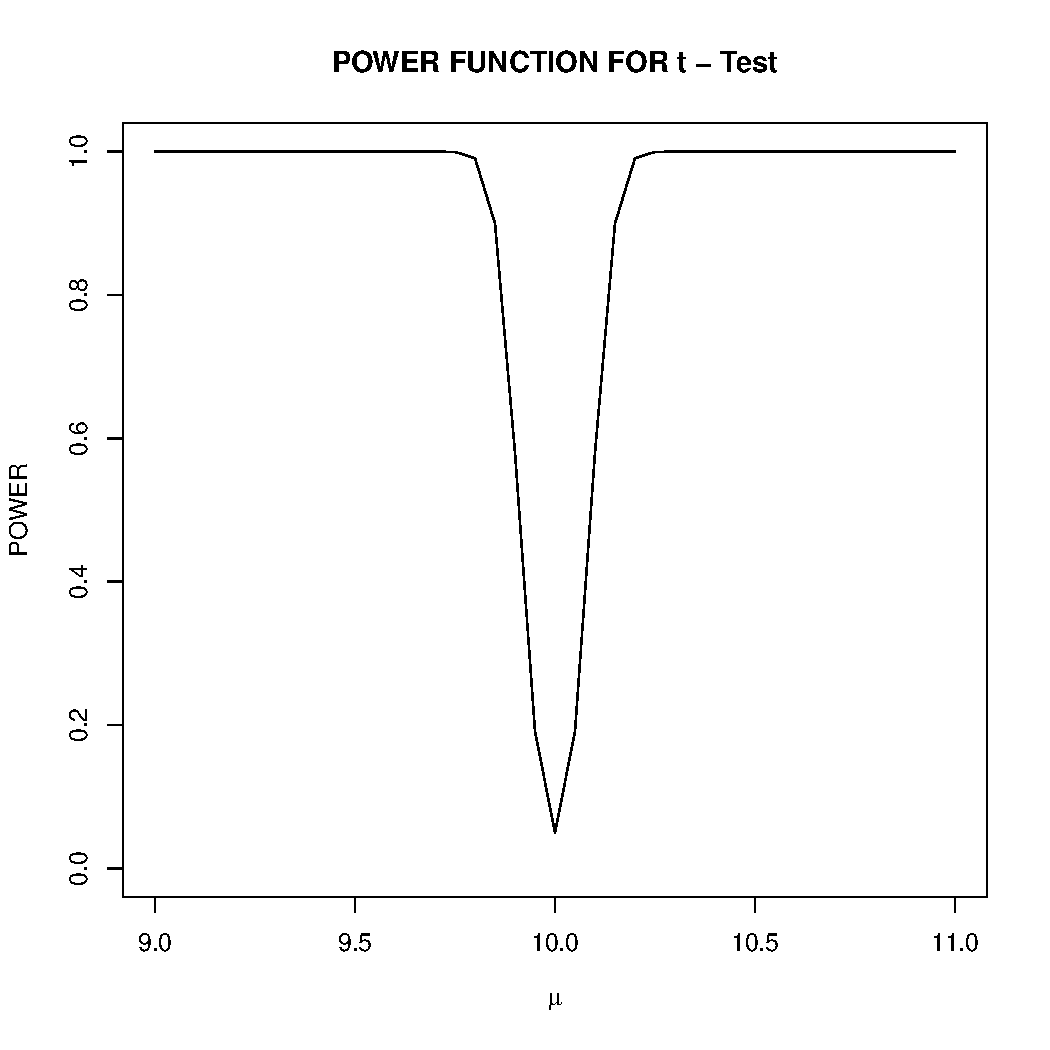
\includegraphics[width=0.8\textwidth]{Rplots.pdf}
\end{figure}
\newpage
The R code is: \\
\begin{verbatim}
n = 36
df = n-1
muo = 10
sigma = .27
mu = seq(9,11,.05)
delta = sqrt(n)*(mu-muo)/sigma
power = 1-pt(qt(.975,df),df,delta) + pt(qt(.025, df), df, delta)
#par(lab=c(15,20,4))
plot(mu,power,type="l",ylim=c(0,1),xlab=expression(mu),
ylab="POWER")
title("POWER FUNCTION FOR t - Test")
out = cbind(mu,delta,power)
\end{verbatim}
The sample mean is 10, so our $T$ statistic is 0, thus $G$ is centered at 0, so: \\
\begin{align*}
\gamma(\mu) &= G(-t_{.025}) + 1 - G(t_{.025}) \\
&= .025 + 1 - .975 \\
&= .05
\end{align*}
\item To determine the sample size, we have $\alpha = .05$, $\beta = .2$, and $\phi = \frac{.2}{.27} = 0.7407$. From the table $A11$, this gives us a sample size of $13$. \\
\end{enumerate}
\section*{Problem 2}
\begin{enumerate}
\item The null hypothesis is $\mu \geq 5$, with the alternative hypothesis being $\mu < 5$. \\
$\sigma$ is unkown, so we will be using t testing. \\
We know that: $n = 20$, $\hat{\mu} = 4.2$, $S = 1.2$, and $\alpha = .05$, so we have the T statistic: \\
\[
T = \frac{\sqrt{20}(4.2 - 5)}{1.2} = -2.98142396999972
\]
the t critical value is: \\
\[
t_{.05} = -1.729
\]
(from the table). \\
Since $T < t_{.05}$, we reject the null hypothesis. We also have the p-value for $T$ which is approximately $.005 < .05$ from the table. \\
\item The probability that the test will be able to detect that the real mean is 4.1 or less can be given by the power function [ ]
\[
\gamma(\mu) = G(-t_{.05})
\]
where $G$ is the cumulative t distribution centered at $\delta = \frac{\sqrt{20}(4.1 - 5)}{1.2}$ with $df = 19$. This can be solved with R: \\
\begin{verbatim}
result = pt(-qt(.05, 19), 19, 0.3727)
\end{verbatim}
which yields a power of 0.9006489
\item For sample size estimation we know: $\alpha = .05$, $\beta = .1$, and $\phi = \frac{|4.4 - 5|}{1.2} = .5$. From the table this gives us 44
\end{enumerate}
\section*{Problem 3}
\begin{enumerate}
\item We will assume the population distribution is normal, since this is a manufacturing process. \\
The null hypothesis is that $\sigma \geq 1$, the alternative hypothesis is that $\sigma < 1$. We can calculate the test statistic: \\
\begin{align*}
TS &= \frac{(n - 1) * S^2}{\sigma_o} \\
&= \frac{19 * .8458^2}{1} \\
&= 13.5922
\end{align*}
we can determine the critical value with: \\
\begin{align*}
t_{.05} &= \chi_{19, .95}^2 \\
&= 10.117
\end{align*}
The test statistic is not less than the critical value, thus we fail to reject the null hypothesis. \\
\item We have the power function: \\
\begin{align*}
power &= G(\frac{\sigma_o^2}{\sigma_1^2}\chi^2_{n - 1, 1 - \alpha}) \\
&= G(10.117) \\
&= .05 \\
\end{align*}
so the type II error rate for $\sigma_1 = 1$ is $1 - .05 = .95$. For $\sigma_1 = .9$: \\
\begin{align*}
power &= G(\frac{\sigma_o^2}{\sigma_1^2}\chi^2_{n - 1, 1 - \alpha}) \\
&= G(\frac{1^2}{.9^2}\cdot 10.117) \\
&= G(12.4901) \\
&= 0.1363781
\end{align*}
so the type II error is 0.8636219. For $\sigma_1 = .8$: \\
\begin{align*}
power &= G(\frac{\sigma_o^2}{\sigma_1^2}\chi^2_{n - 1, 1 - \alpha}) \\
&= G(\frac{1^2}{.8^2}\cdot 10.117) \\
&= G(15.81) \\
&= 0.32994
\end{align*}
so the type II error is 0.67006. For $\sigma_1 = .7$: \\
\begin{align*}
power &= G(\frac{\sigma_o^2}{\sigma_1^2}\chi^2_{n - 1, 1 - \alpha}) \\
&= G(\frac{1^2}{.7^2}\cdot 10.117) \\
&= G(20.6469) \\
&= 0.6433
\end{align*}
so the type II error is .3567. For $\sigma_1 = .6$: \\
\begin{align*}
power &= G(\frac{\sigma_o^2}{\sigma_1^2}\chi^2_{n - 1, 1 - \alpha}) \\
&= G(\frac{1^2}{.6^2}\cdot 10.117) \\
&= G(28.1027) \\
&= 0.918528
\end{align*}
so the type II error is .08147. \\
\item The bound for the upper 90\% CI is given by: \\
\begin{align*}
CI &= \frac{\sqrt{n - 1} \cdot S}{\sqrt{X^2_{1 - \alpha, n - 1}}} \\
&= \frac{\sqrt{19} \cdot .8458}{\sqrt{X^2_{.9, 19}}} \\
&= \frac{\sqrt{19} \cdot .8458}{\sqrt{11.651}} \\
&= 1.0801
\end{align*}
This aligns with my results in part 1 since 1 is included the in the CI. 
\end{enumerate}
\section*{Problem 4}
\begin{enumerate}
\item $S_+ = 5$, so we have: \\
\[
p = G(5, 20, .5) = .021
\]
where G is the cdf of the binomial distribution with $p = .5$, $n = 20$, and $x = 5$. \\
.021 < .05, so we reject the null hypothesis. \\
\item 
\end{enumerate}
\end{document}